% !TeX encoding = UTF-8
% !TeX program = pdflatex
% !TeX spellcheck = en_EN

\documentclass[Lau,binding=0.6cm]{sapthesis}

\usepackage{microtype}
\usepackage[utf8]{inputenx}
\usepackage{listings} 


\lstset{
	keepspaces=true,
	basicstyle=\ttfamily,
	tabsize=2,
	keywordstyle=\color{blue}
}

\usepackage{hyperref}
\hypersetup{pdftitle={spallaccini-tesi-laurea},pdfauthor={Davide Spallaccini}}

% Remove in a normal thesis
\usepackage{lipsum}
\usepackage{curve2e}
\definecolor{gray}{gray}{0.4}
\newcommand{\bs}{\textbackslash}

% Commands for the titlepage
\title{An Intel Pin Tool for dynamic detection\\ of Return Oriented Programming}
\author{Davide Spallaccini}
\IDnumber{1642557}
\course{Ingegneria Informatica e Automatica}
\courseorganizer{Facoltà di Ingegneria dell'informazione, Informatica e Statistica}
\AcademicYear{2016/2017}
\copyyear{2017}
\advisor{Prof. Daniele Cono D'Elia}
\coadvisor{Prof. Camil Demetrescu}
\coadvisor{Prof. Emilio Coppa}
\authoremail{davide.spallaccini@gmail.com}


\begin{document}

\frontmatter

\maketitle

\dedication{Dedicated to\\ Jon Skeet}

\begin{abstract}
In this work we introduce a tool that can be dynamically attached to a running software and through dynamic binary instrumentation and some heuristics is able to detect if a sequence of executed instructions is a result of a Return Oriented Programming attack that diverted the program’s control flow leading to arbitrary code execution.
\end{abstract}

%\begin{acknowledgments}
%[TODO]
%\end{acknowledgments}

\tableofcontents

\chapter{Introduction}
A very large part of security vulnerabilities that afflict modern software is closely related to software bugs that involve a bad use of memory accesses. Some modern programming languages like Java implement a runtime error detection that for example checks array bounds and pointer dereferences. On the other side, lower level languages that allow the programmer to directly interact with memory, like C and C++, may not support any automatic bounds checking and are often referenced as memory-unsafe.
Programs may exhibit different types of memory errors: invalid read or write operations to/from a certain address (buffer overflow, use after free, …), uninitialised variables (null pointer dereference, wild pointers), incorrect or absent tracking of memory usage. An exploitation takes place when an attacker subverts the program control flow so that it performs attacker-directed operations that were not intended by the program.
The most familiar vulnerability classes are stack overflow, heap buffer overflow, integers overflows, and format string vulnerabilities.
An attacker can detect that some software suffers of certain bugs and can rely on a wide range of exploitation techniques to hijack the control flow and finally execute malicious code.

\section*{List of Contents}
In chapter 1 we will revise the fundamentals of buffer overflow vulnerabilities describing modern defences against such threats, then we will explain how a return-to-libc attack works and how return oriented programming is an advanced version of that technique. In chapters 2 and 3 we will present our idea and the details about the implementation, we will also explain what is Intel Pin tool and how it helped in the implementation of the idea. In chapter 4 we will describe the experimental aspects of my work, including tests on real world exploits and Windows applications. Finally we will evaluate some future directions and possible problems and improvements of my work.

\mainmatter

\chapter{Technical Background}

In this chapter I will discuss my stylistic choices of \textsf{sapthesis}.
I will show the page layout geometry and I will describe the page style.

\section{Basic Concepts}

Before we continue I’d like to point out some basic (if not obvious) definitions:
\begin{itemize}
\item
buffer/stack: a buffer is a contiguous block of computer memory that contains data of the same nature. A stack is a commonly used abstract data type which has the property that the last object added to a stack (push instruction) is the first that will be removed (pop instruction).
\item
control flow: it is the order in which different statements are executed. It is determined by sequence of branches taken by a certain program. Is a distinctive characteristic of imperative languages, as opposed to declarative languages.
\item
shellcode: is a sequence of low level instructions encoded as a string of bytes. It is called in this way because traditionally its purpose is to spawn a new shell for the attacker use. A peculiarity is that since shellcode is contained in exploiting payloads, it tends not to use null bytes that could work as string terminators for example, adding some constraints to the coding of certain operations. 
\item
EIP/return address: when a function is called through the call instruction, before executing the function code the processor must “remember” what to do after the function returns. To do this the processor stores the address of the next instruction to execute pushing it on the stack before setting up the memory for the function. EIP is the name of the register that contains the address of the next instruction to execute.
\item
stack pointer/frame pointer: the stack pointer points to the top of the stack. In particular in x86 the ESP register contains the value at which the last element on the stack is stored. The frame pointer is a fixed reference point inside a function frame on the stack. It serves as a facility to locate more efficiently parameters and local variables inside a function, and in fact it’s not strictly necessary.
\end{itemize}


A process memory is organised in three main logical regions: code segment, data segment, stack segment.
The code memory region contains all the instructions of the program, the instruction pointer contains the address of the next instruction to be executed, this region is normally marked as read-only . The data segment contains initialised and uninitialised variables and dynamic buffers (heap region). The stack contains the function frames which in turn contain function local variables, function arguments, and different pointers (to the stack top, to the frame and to the return address). In this work I’ll assume that the base of the stack is located at some fixed address, and that it grows down, i.e. towards lower memory addresses.


In high level languages a paramount abstraction is the function, and functions use the stack, so a key concept is to understand how do they work. At the assembly level, before calling a function its parameters are pushed on the stack. Then the call instruction is executed; note that this is equivalent to pushing the value of EIP (that at the moment is the statement after the call in the calling function) on the stack and jumping to the first instruction of the called function. The prologue of a function sets up the frame and the frame pointer (on Intel’s CPUs BP (EBP) is used for this purpose) so that local variables can be created and easily accessed on the stack. The frame is essentially the region on the stack containing parameters, the saved EIP and local variables of the function. The epilogue cleans up the frame and restores the previous frame pointer. The ret instruction is equivalent to popping the saved EIP back in it’s place so that the control returns to the instructions after the call.




\section{Stack Smashing: buffer overflow vulnerabilities attacks and defences}

Let’s consider the situation in the diagram in Figure 1.1 representing the memory layout of a simple function. As we can see the function takes two parameters as input and allocates a local buffer of dimension N. 
Let’s suppose that the parameters are a pointer to an input buffer and its dimension and that the input data is copied to the local buffer. This last operation can be really dangerous. Without some strong bounds checking on the input and destination buffers the code that writes data in the local buffer may overwrite the memory locations containing the old frame pointer and the saved EIP. This means that after the frame cleaning up when the ret instruction will be executed the following instruction will be fetched from the address that was written by the buffers copy operation.  
\begin{figure}
\centering
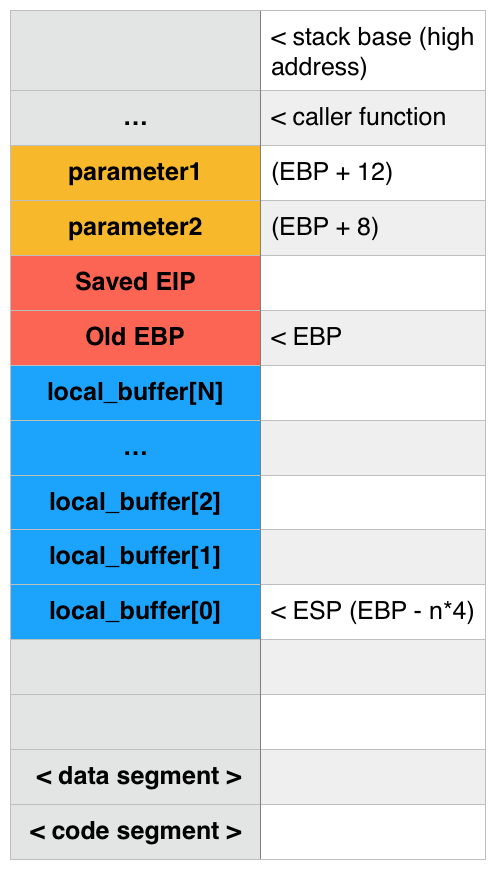
\includegraphics[width=0.42\textwidth]{overflow}
\caption{Stack configuration before stack buffer overflow}
\label{fig:largenenough}
\end{figure}
An attacker can take advantage of the situation devising a particular input that overwrites the EIP with his own address. Depending on the address that the attacker decides to put instead of the original one different types of attack are carried out.
In the classic version of the attack the malicious code is written inside the input payload. After the buffer overflow the EIP is overwritten with an address that points to the malicious code that was previously copied on the stack. This malicious code is usually not so long and is commonly known as shellcode, even if it doesn’t necessarily spawn a shell. Another way to include shellcode in a process image is to write it in an environment variable, in that case the attacker again needs to know where this variable is stored.


Modern systems implement some effective countermeasures to this approach.
One of these defences are stack canaries that try to ensure that critical memory locations are not overwritten, and try to prevent stack overflows problems at the root.
Another important defence is called Data Execution Prevention, or Write Xor Execute, or Exec Shield (the name depends on the system the measure is implemented in). This defence partitions the memory locations in writable (data) and executable (instructions), so no location is both, the defence is based on the fact that program’s data, especially input data, in general should not be executed while the program is running. Of course there are special cases where this is required by the nature of the program [e.g. ???]. This is carried out both in software and in hardware. In modern CPU technologies one of the bits of memory addresses indicates whether the page is marked as executable (code memory pages) or not (stack, heap, etc.), this means that information in a certain page can be executed (instructions) or written (data) but not both. Before hardware support this feature was emulated at software level with the technologies named before.


Another defence is called Address Space Layout Randomisation or ASLR. For a buffer overflow exploit to be reusable the attacker needs to know the exact address (or at least a narrow interval of addresses) that he has to overwrite in the saved EIP location. With ASLR the base addresses of stack, heap and libraries are randomly rearranged at loading time, so that the attacker can’t guess the actual address his malicious payload will be put. This type of defence makes buffer overflow exploitation extremely unlikely to succeed on 64-bit machines, on the other side on 32-bit machines typically only 16 bits are available to randomisation, which means that the attacker can use brute force and guess the base addresses he needs in a 
matter of minutes.


\section{Ret-to-libc}

For the attacker one of the first obstacles to overcome is to find a way to execute malicious code. If programs are protected with DEP or W \textasciicircum X this may be difficult as the only code that can be executed is the one that is already part of the program when it is loaded.
The return-to-libc is a method to bypass the W \textasciicircum X defence in linux systems which allows the attacker to reuse the code already present in libc (libc is targeted since it’s present in almost every Unix program) to execute unintended activities. Of course the attacker is limited by the code actually present in the library, but this is often enough to carry out a serious attack.


The attack consists in creating a fake stack configuration emulating the typical steps of code that prepares a call to the desired libc function. In particular the called libc function will expect that its arguments are pushed in reverse order and that the return address is memorised at the top of the stack by the call instruction.   
This can be easily done extending the buffer overflow process. In fact after overwriting the saved EIP, additional data must be put on the stack to craft the desired function arguments plus return address. The overwritten return address will be the address of the first instruction of the desired libc function (most of the times you’ll want to call something like system(“bin/sh”) ).  


As you can see with the same mechanism the attacker can craft the stack so that a chain of  functions can be called allowing more complex operations to be executed. All he need is to choose the second return address and arrange the new parameters for the next function to call.
One of the main mitigations to this threat is to remove some libc functions from the program address space if they are not needed, this can significantly weaken the attack chances to succeed.

\begin{figure}
\centering
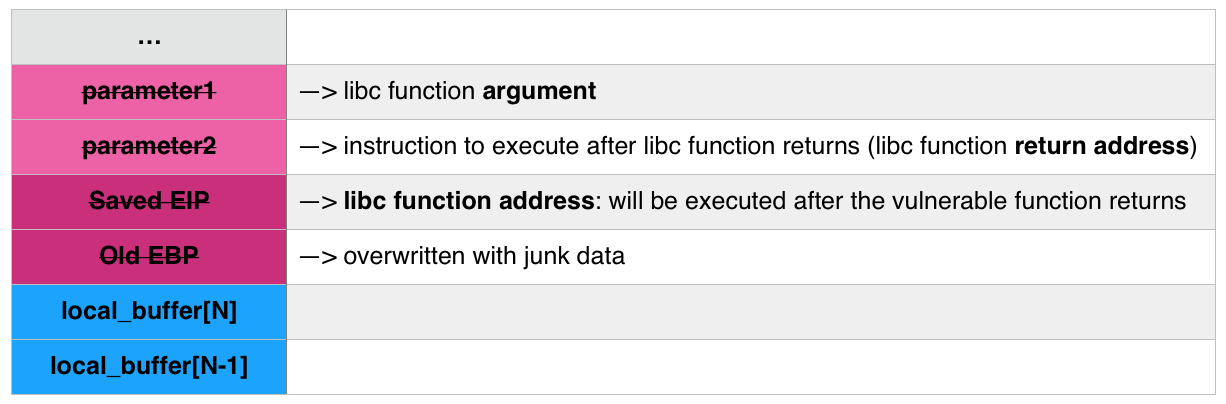
\includegraphics[width=0.7\textwidth]{ret-to-libc1}
\caption{Ret-to-libc: stack configuration during overwriting}
\label{fig:largenenough}
\end{figure}

\begin{figure}
\centering
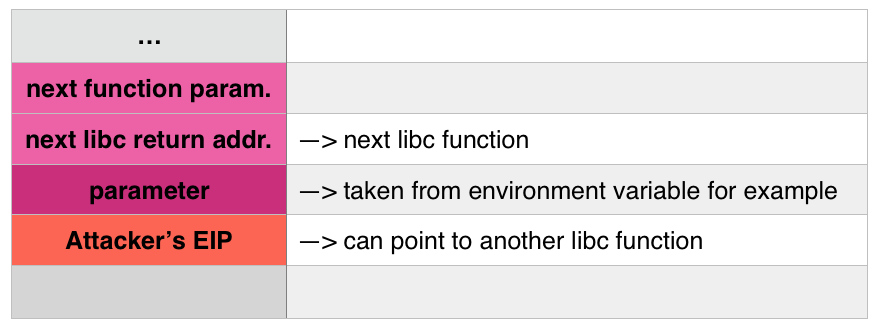
\includegraphics[width=0.5\textwidth]{ret-to-libc2}
\caption{Ret-to-libc: stack configuration right before the call to libc function}
\label{fig:largenenough}
\end{figure}

\section{Return Oriented Programming}

“We challenge the flawed, but pervasive, assumption that preventing the introduction of malicious code is sufficient to prevent the introduction of malicious computation.” (Shacham et al.)

\begin{figure}
\centering
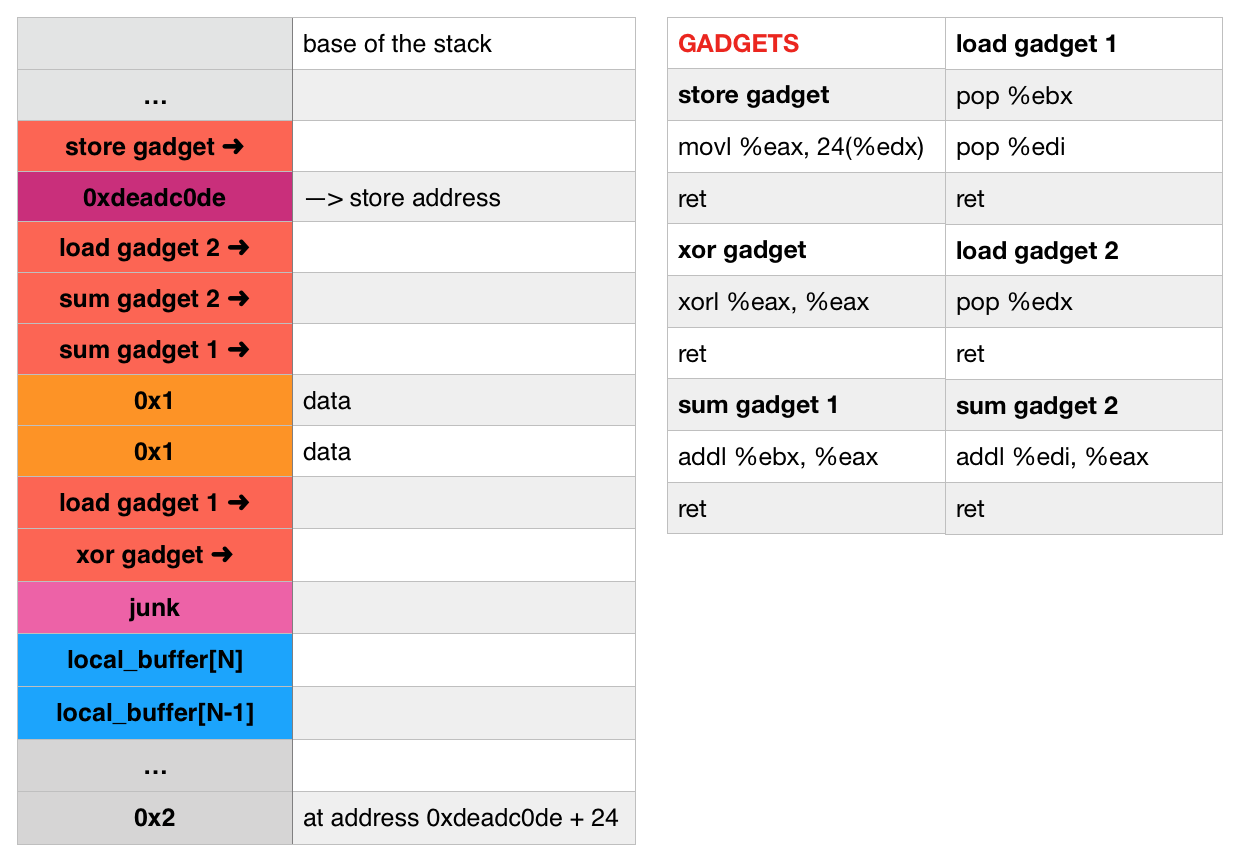
\includegraphics[width=1\textwidth]{ropadd}
\caption{Addition through a ROP chain}
\label{fig:largenenough}
\end{figure}

Return oriented programming extends from the ideas behind the ret-to-libc attack. A major characteristic of this attack is that it categorically bypasses W\^X protections and in general any defence that excludes the chance to inject malicious code. At the same time, in theory, the attacker is allowed to execute arbitrary computation, since ROP creators provide proof that a Turing-complete toolset can be built in sufficiently large programs. 
This means that even with modern memory protections any malicious behaviour is achievable just by reusing code already present in the target program.
The main organisational unit of a ROP attack is an arrangement of data on stack that the originators of this technique call gadget, a gadget typically ends with an instruction address.


This instruction address points to a short sequence of instructions ending in a ret. These short sequences use the data that the attacker puts on the stack and save the result of the computation on the stack itself or in registers. When the last instruction, that is a ret, is executed the address of the next short sequence of instructions is popped from the stack into the instruction pointer, so the ROP program continues. 
This succession is what is called a ROP chain, in other words a chain of short instructions sequences ending in a ret linked together by stack operations.
The purpose of each gadget is to accomplish elementary computations like arithmetical or logical calculations, load and store operations or conditional jumps.


So, like return to libc attacks, ROP uses the stack and the stack pointer as a mean to chain together different steps of an action.
When crafting an attack one of the main issues is to find the right sequence of function fragments ending in a ret so that the right higher level operations are executed, for this reason often the term gadget is referred to these function fragments rather than to the organised memory locations in the stack as in the original paper. In this work I will follow this habit.
  

Let’s do an example of a simple sum computation using Return Oriented Programming.
Let’s suppose that the ROP attack is triggered by a stack overflow. Now let’s follow the sequence of the events. All the payload is written on the stack, eventually overwriting earlier data. In particular the saved EIP location of the vulnerable function is overwritten with the address of the first gadget. 
To better understand the dynamics of what is going on here recall that ret is equivalent to pop \%eip. In this example after the vulnerable function returns, the first instruction of the xor gadget is executed. When the ret is reached, the processor pops the address of the load gadget from the stack into \%eip, so the load gadget is executed.
As you can see this gadget expects data on the stack to be put in the registers. Once again the ret mechanism gives the control to the next gadget. The sum gadgets are chosen after the load gadget and rely on the fact that the \%edi and \%ebx registers were not modified by eventual gadgets that could have been executed after the load operation. The logic of the final store operation at this point is quite straightforward. (Notice that this is just a simple example, there’s no guarantee that you can always find such convenient gadgets and operations can get really tangled if no good gadgets are given with the executable).


\section{Using ROP to disable DEP in Windows}

In practice the aim of a ROP attack is typically to change the protection policies of the memory location where the shellcode is loaded, for example through a call to mprotect() in Unix or VirtualProtect() or SetProcessDEPPolicy() on Windows. In the following paragraphs we will recall some notions about Windows DEP settings and bypassing techniques.


As said before when hardware DEP is enabled you cannot jump to your shellcode, because it will not be executed. Instead, the attempt will trigger an access violation, with the subsequent process termination.
In the Windows operating systems there are 4 possible DEP configurations that are named as follows:
\begin{itemize}
\item
OptIn: On systems with processors that can implement hardware-enforced DEP, DEP is enabled by default for limited system binaries and programs that "opt-in." With this option, only Windows system binaries are covered by DEP by default. 
\item
OptOut: All processes, services in the system are protected by default. You can manually create a list of  exceptions that “opt-out” one or more programs from DEP protection.
\item
AlwaysOn: The same protection as OptOut but no exceptions are allowed.
\item
AlwaysOff: DEP is turned off, regardless of hardware support.
\end{itemize}

In addition to those 4 modes, MS implemented a mechanism called "Permanent DEP", which uses SetProcessDEPPolicy(PROCESS\_DEP\_ENABLE) to make sure processes are DEP enabled. On Vista (and later), this "permanent" flag is automatically set for all executables that were linked with the /NXCOMPAT option.
The default DEP configurations in the various Windows system versions are the following:
\begin{itemize}

\item Windows XP SP2, XP SP3, Vista SP0 : OptIn
\item Windows Vista SP1 : OptIn + Permanent DEP
\item Windows 7/8/10: OptIn + Permanent DEP
\item Windows Server 2003 SP1 and up : OptOut
\item Windows Server 2008 and up : OptOut + Permanent DEP

\end{itemize}

Under Vista, Windows 2008, Windows 7, you can change the configuration using the bcdedit command :
\begin{verbatim}
bcdedit.exe /set nx OptIn
bcdedit.exe /set nx OptOut
bcdedit.exe /set nx AlwaysOn
bcdedit.exe /set nx AlwaysOff
\end{verbatim}

Notice that if DEP is turned off, there’s nothing to defeat, so ROP is not required as traditional shellcode can be executed. If DEP is turned on you can choose to completely rewrite your malicious code in a ROP manner, or you can try to bypass the current DEP protection with the help of some particular Windows APIs. In the second case the ROP payload will attempt to set up the stack for the desired function and through it make the memory where the shellcode will be located executable. The most useful functions to accomplish this job are:
\begin{itemize}

\item VirtualAlloc
\item HeapCreate
\item SetProcessDEPPolicy
\item NtSetInformationProcess
\item VirtualProtect
\item WriteProcessMemory

\end{itemize}

Each of these requires its own adaptation and precaution, and not all of them are compatible with all the System / configuration combinations. Refer to the table below as a compatibility reference.

\begin{figure}
\centering
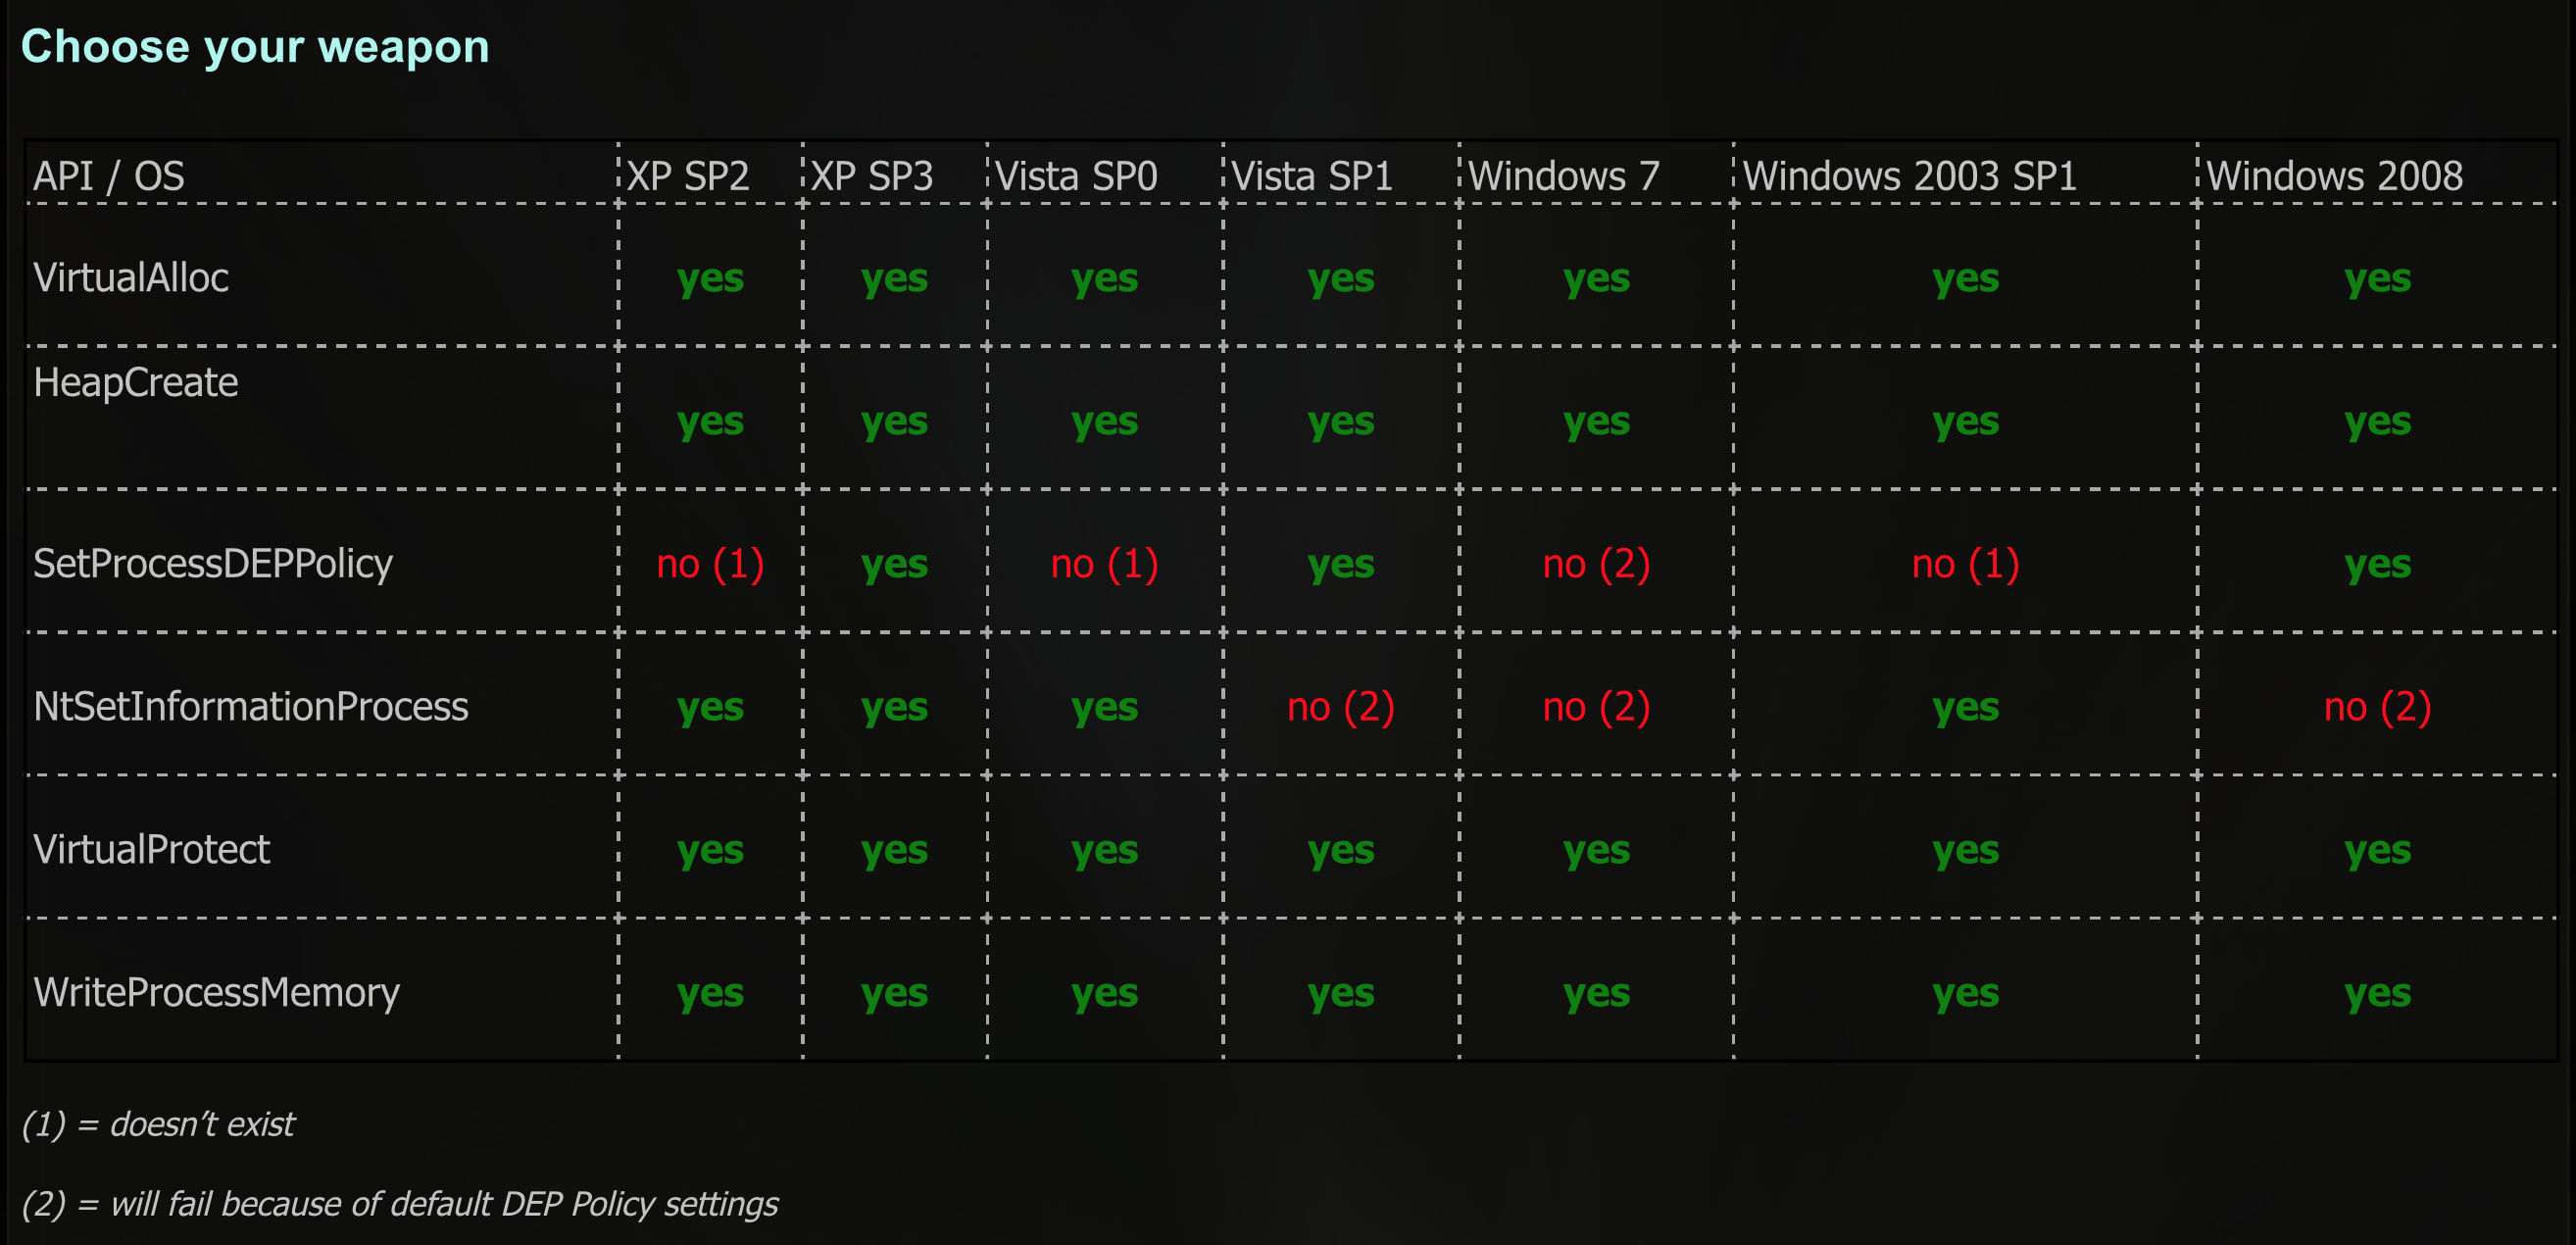
\includegraphics[width=1\textwidth]{windepapi}
\caption{Ret-to-libc: stack configuration right before the call to libc function}
\label{fig:largenenough}
\end{figure}

\chapter{Design}

In this chapter I will describe the design and some of the heuristics we used to implement the tool.

\section{Problem definition}

The problem we decided to face is to see if it is possible to detect at runtime, through dynamic binary instrumentation, if a ROP attack is running in a target program. Since the code that is executed in this type of attack is actually legal code taken from legal memory locations you need some insight on the latest instructions that were executed and try to understand if the code is behaving in an unexpected manner. This type of insight can weigh on performance, since you have to get at least some information about the nature of each instruction, so the detection checks should be agile and quick. At the same time we want to make sure that the developed analysis doesn’t actually stop the normal course of everyday applications: this means that we have to be really careful in choosing the right parameters when trying to distinguish between legal execution and ROP attack.

\section{Existing ROP mitigations and defences}

Several defences against ROP and ret-to-libc have been developed in the last years. Some of these defences are based on some mitigations to be applied during compilation, for example in the case of ret-to-libc at linking time dangerous functions that are not used by the program can be removed from the address space. To hamper ROP some researchers have devised a new approach they called G-Free that claims to be able to eliminate unaligned free-branch instructions, and to protect the aligned free-branch instructions to prevent them from being misused by an attacker. In practice they employ mechanisms to check that a function is being entered from its proper entry point. Other rather popular defences target legacy binary software, and do not require, if not in minimal part, any binary code rewriting. The most notable defence tools available are kBouncer and ROPGuard for Windows and ROPecker for Linux. kBouncer received broad attention not only from the research community when its first version was announced as the \$200,000 winner of the Microsoft BlueHat Prize. ROPGuard placed second at the BlueHat Prize and has since been incorporated into Microsoft’s Enhanced Mitigation Experience Toolkit (EMET) [it is based on this technique… ]. ROPecker was introduced in 2014 and has the characteristic of being very light and efficient [what deos it do?]
gadget-less binaries

\section{Tool overview}

Since the typical attack often targets a determined set of system calls with the purpose of changing memory protection policies, one of the ideas could be to check in the neighbourhood of these functions if something unexpected is happening, however since ROP is not closely related to these system calls (recall that the original ROP paper even talks about ROP shellcode), we can start with a solution that actually looks at the executed code.
In the design session of the work we initially observed that one of the most distinguishing features of ROP is the abundant use of ret instructions that in fact work as links between micro operations. So the main metric we chose to detect ROP is to check how large is the distance between the ret instructions from the last cluster.
To test my ideas we wrote a simple Intel Pin tool (I will talk about Pin and dynamic instrumentation in more details later) that disassembles the executed instructions together with additional information about the instruction address and source library, printing a trace of a program execution. Then we analysed the resulting files with python scripts implementing a prototype of the idea.
In the following paragraph we will display the different steps and heuristics that we devised before getting to the final implementation of the tool.

\section{Version 0.1}

In the first version of the tool we introduced the main data structure that collects the informations about the executed instructions before running through the various detection tests.
This data structure is a fixed size list of integers, the elements are maintained as in a FIFO: the newest information gathered from the program execution replaces the oldest one. Of course the sizing of the list is a critical parameter. 


In this first version the list maintains the number of executed instructions between two consecutive rets, for the last N ret instructions.


Example: 

\begin{lstlisting}
N = 3

1 - mov eax, dword ptr [eax]			list = []
- - ret														list = [1]
1 - push eax											list = [1]
2 - add dword ptr [ebp+0x5], esi	list = [1]
3 - push 0x1											list = [1]
4 - pop eax												list = [1]
5 - pop esi												list = [1]
- - ret														list = [1, 5]
1 - mov edx, 0xe58b0001						list = [1, 5]
2 - pop ebp												list = [1, 5]
- - ret														list = [1, 5, 2]
1 - pop ebx												list = [1, 5, 2]
- - ret														list = [5, 2, 1]
1 - add edx, ebx									list = [5, 2, 1]
2 - pop ebx												list = [5, 2, 1]
- - ret 0x10											list = [2, 1, 2]

\end{lstlisting}

After all this information is collected, every time an old interval length is removed from the list, the detection routine is called to check the current situation.
[How does the detection algorithm work?]
The basic check is described by the following code:

\begin{lstlisting}[language=Python]
def too_short_intervals(intervals):
    threshold = 3
    percent = 90
    short_intervals = 0
    for i in intervals:
        if(i < threshold):
            short_intervals += 1
    if((short_intervals/len(intervals)) > percent/100):
           return True
    return False
\end{lstlisting}

Basically we are checking if in the current list there are a certain percentage of ret instructions that are too close to each other. However even with simple tests this first idea suffers of some false positives. This happens because a crowding of ret instructions, although rare, it’s not itself completely illegal as sequence of instructions, in fact some low level or system API sometimes present this kind of behaviour.
Notes on the distances buffer dimensioning
If the size is too short there may be some particular situations in legal code where there are return instructions really close to each other (e.g. a short recursive function). On the other hand if the size of the list is too large the information may become noisy, in the sense that if the attack code is much shorter than the list size (one of the examples executes the attack using only 11 gadgets) when analysing the disposition of instructions, the presence of too much legal code information in the list makes the detection operations harder and too ambiguous.
Let’s make this clear through an example.


[5, 11, 7, 12, 12, 20, 15, 9, 10, 10, 10, 0, 1, 1, 2, 1, 1, 1, 1, 5, 2, 1, 2, 0, 1, 2, 2, 1]
(the attack is in bold)


In this case the size of the list is 28. The attack covers about the 60\% of the list, so a detection heuristic should be able to detect that only part of the information is irregular. At the same time the detection routine should be able to recognize the grouped disposition of short instruction sequences ending with ret. To show this let’s shuffle the list above:


[12, 1, 10, 2, 20, 15, 0, 1, 7, 1, 5, 2, 1, 1, 0, 11, 1, 1, 2, 2, 1, 12, 9, 10, 5, 2, 1, 10]


In the ROP practice, as we will also point out later, it’s really unlikely that a gadget of more than 7 or 8 instruction is executed, because very long gadgets cause the ROP computation to be much more difficult to achieve by overcomplicating the stack management and hindering the already tangled control flow.
So, even if the values of the distances are the same in the two lists, the second situation is not to be considered a possible ROP execution trace since the short intervals are too scattered across the list. This means that the detection routine should be able to recognize patterns in the collected data to recognize the ROP payloads. This can be avoided tough with a good dimensioning of the list that must not be too much larger than the shortest attacks present in the real world. As we will point out in the implementation section, we observed a really short ROP payload containing only 11 gadgets, so we chose a dimension of 14 (in the following versions we will explain how we managed that +3 additional elements). At the same time in fact the list cannot be too short otherwise some legal code sequences could be misinterpreted as ROP chains.

\section{Version 1.0}

Examining the first false positives from version 0.1 we noticed that it was not so uncommon for ret instructions to be 2 or three instructions away from each other. In particular we observed that in some libraries of the first vulnerable application under test there was a pattern of instructions repeated many times consecutively, the pattern is composed of these instructions:


\begingroup
    \fontsize{8pt}{9pt}\selectfont
\begin{verbatim}

0x75ad3eee C:\Windows\system32\urlmon.dll:.text+0x10d69        push 0x75b8e4b8
0x75ad3ef3 C:\Windows\system32\urlmon.dll:.text+0x10d6e        call dword ptr [0x75ac18ac]
0x75ad3ef9 C:\Windows\system32\urlmon.dll:.text+0x10d74        ret 
0x75ad3edd C:\Windows\system32\urlmon.dll:.text+0x10d58        push 0x75b8e4d0
0x75ad3ee2 C:\Windows\system32\urlmon.dll:.text+0x10d5d        call dword ptr [0x75ac18ac]
0x75ad3ee8 C:\Windows\system32\urlmon.dll:.text+0x10d63        ret 
0x75ad3ecc C:\Windows\system32\urlmon.dll:.text+0x10d47        push 0x75b8e3f8
0x75ad3ed1 C:\Windows\system32\urlmon.dll:.text+0x10d4c        call dword ptr [0x75ac18ac]
0x75ad3ed7 C:\Windows\system32\urlmon.dll:.text+0x10d52        ret 
0x75ad3ebb C:\Windows\system32\urlmon.dll:.text+0x10d36        push 0x75b8e458
0x75ad3ec0 C:\Windows\system32\urlmon.dll:.text+0x10d3b        call dword ptr [0x75ac18ac]
0x75ad3ec6 C:\Windows\system32\urlmon.dll:.text+0x10d41        ret 

\end{verbatim}
\endgroup


What we improved in this second version is the introduction of a new heuristic that deals with such false positives. In particular we noticed that in a regular program all the input data that the attacker wants to pass to his program must be overwritten on the stack, for example after a buffer overflow, and then loaded from there into registers. Even if the attacker just wants to call a system API function he has at least to load into registers the function’s parameters. As pointed out in the original paper of ROP, the constant loading operations and the loading and storing from/to memory operations of a computations are performed with gadgets of the form:

\begin{lstlisting}[language={[x86masm]Assembler}]
pop %register             #Constant loading
ret

movl %eax, 24(%edx)       #Store to memory
ret

movl 64(%eax), %eax       #Load from memory
ret
\end{lstlisting}


All these operations have in common the fact that the gadget is composed by only two instructions one of which is the ret. 
As said before we expect in a ROP execution to find at least a consistent number of constant loading operations. We could have checked for the presence of pop-ret or movl-ret sequences inside a suspect execution trace but to keep the detection fast and simple we opted for the introduction of a second threshold in the detection routine. The first threshold from version 0.1 of the tool checked if there were too few instructions between two consecutive rets, and checked if this this event happened too often in a given analysis window. In terms of the list of intervals the detection routine checked if a given percentage of elements were below the threshold value.
This new threshold does the same type of check but in a more restrictive way. In fact its purpose is to detect the presence of load/store gadgets. The detection provides a positive result if the two checks for the two thresholds are hit at the same time.


So adding a second threshold is the core when scanning the distances list. This threshold checks the presence of ret instructions that are at a distance of one executed instruction or less. At the same time the percentage related to this second threshold has to be more relaxed, since the detection logic must take into account the presence of other calculations that are different from load/store and that hence may require the use of longer gadgets. So the detection routine is modified like this:

\begin{lstlisting}[language=Python]
def too_short_intervals(intervals):
    threshold = 3
    percent = 90
    threshold2 = 2
    percent2 = 50
    short_intervals = 0
    very_short_ints = 0
    for i in intervals:
        if(i < threshold):
            short_intervals += 1
        if(i < threshold2):
            very_short\_ints += 1
    cond1 = (short_intervals/len(intervals)) > percent/100
    cond2 = (very_short_ints/len(intervals)) > percent2/100
    if(cond1 and cond2):
           return True
    return False
\end{lstlisting}

Note that to get to the current values for the thresholds and percentages we had to check the effectiveness on different types of attacks and tests targeting false positives in large real world applications.

\section{Version 2.0}

Version 1.0 was quite accurate in detecting an attack in a known exploit while not showing false positives in the vulnerable applications under test, however when testing larger applications like Mozilla Firefox, we found that there were some libraries that exhibited some sequences of instructions with a dense crowding of ret instructions very close to each other. This of course was detected by the script so some additional criteria were needed to recognise the attacks. 


For this purpose we had to consider further characteristics of the code executed by a ROP attack. In particular we tried to focus on the addresses of ROP instructions. Of course, since ROP is a code reuse attack all of this addresses are legal and belong to different functions. At the same time, since ASLR is one of the sworn enemies of ROP, we expect that all the addresses are taken from some library that was not under the effect of ASLR. However even ASLR can be bypassed, in that case the base address of some library may have been leaked, but in any case you may expect that the attack will use gadgets all taken from that library.


This may lead you to think that the addresses of a certain ROP attack instructions are taken from a limited range of addresses, like in a normal program. Actually what ROP misses is the memory locality of the instructions that a normal program exhibits. For example consider a brief recursive function that has very few instructions. In this situation if tail recursion optimization isn’t enabled probably the execution trace of the function will contain ret instructions really close to each other, however this is clearly not an attempt to make a ROP exploit. The difference between ROP and this particular situation is, as mentioned before, the level of memory locality. A recursive function will execute the ret instruction fetched almost always from the same memory location, on the other side, since ROP depends on chaining different gadgets from arbitrary memory locations, it will execute ret instructions from points mostly far from each other.


So it is likely that ROP will exhibit in a short sequence of instructions large distances between their addresses. 
Version 2.0 of the script also considers the address of each instruction and compares the addresses of the encountered rets (the instructions between the rets in a ROP attack will reside at a little offset from them). In particular it will store in a list equivalent to that of ret distances, the absolute value of the distances, this time in terms of address, between subsequent rets. The analysis routine scans the input array containing these distances and checks is a good percentage of those are above an experimental threshold distance.


Finally an additional check that is carried out is that in the sequence of instructions that may be considered as a ROP chain the maximum distance in terms of executed instructions is not above a certain threshold. The logic behind this is that it’s really not likely that a ROP chain contains a really long gadget. At the same time it’s not likely that the very long no-ret sequence is in the middle of the list breaking in two halves a ROP chain candidate. In fact this would mean that the second half has lost all the job done by the previous chain, and if the two chains are not detected by the sliding window this means that singularly they were far too short to generate an attack. All of this does not exclude that a ROP chain has less gadgets than the sliding window size, but in that case, for the window motion direction, the long no-ret sequences would be at the end of the list.
I’ll show this with some examples taken from my tests (Mozilla Firefox standard run and Audio-Converter 8.1 under ROP attack):


[ 1, 2, 6, 1, 1, 17, 1, 12, 1, 1, 1, 49, 1, 1 ]


[ 1, 1, 1, 1, 1, 1, 1, 7, 52, 1, 1, 1, 1, 12 ]


In these cases, as you can see, there is a considerable number of ret instructions that are really near to each other (remember 1 means that ret <other instruction> ret is executed). Let’s suppose that there is also a suspect amount of large address differences between subsequent ret instructions. If a ROP attack is running in these instructions there are three possible options:
* there are gadgets of length 17 or even 49 and 52, that is unlikely
* the attack only needs 5 to 8 gadgets, that is possible but still really difficult to find in the real world
* the execution under test is not a ROP attack


[ 1, 1, 1, 1, 1, 1, 1, 1, 1, 1, 0, 190, 290, 45 ]


This on the other hand is an example taken from a real attack that was detected by the version 2.0 tool. As you can notice the number of gadgets in the attack is very low (11 gadgets), but those gadgets are grouped in a compact chain. However this list still exhibits long gadget candidates, but this time they are located at the end of the list when the ROP alert is fired.


The detection routine of this new heuristic looks like this:

\begin{lstlisting}[language=Python]
def far_instructions_seq(address_dists):
    percent = 49
    large_dists = 0
    for i in address_dists:
        if(i > 0xfff0):
            large_dists += 1
    if((large_dists/len(address_dists)) > percent/100):
        return True
    return False
\end{lstlisting}

The previous one instead is modified as follows:

\begin{lstlisting}[language=Python]
def too_short_intervals(intervals):
    threshold = 3        
    percent = 90
    threshold2 = 2
    percent2 = 50
    max_gadget_len = 16

    short_intervals = 0
    very_short_ints = 0
    indx = 0
    for i in intervals:
        if(i < threshold):
            short\_intervals += 1
        if(i < threshold2):
            very_short_ints += 1
        if(i > max_gadget_len and indx not in [10, 11, 12, 13]):
            return False
        indx += 1
    cond1 = (short_intervals/len(intervals)) > percent/100
    cond2 = (very_short\_ints/len(intervals)) > percent2/100
    if(cond1 and cond2):
           return True
    return False
\end{lstlisting}

\chapter{Implementation}

Code instrumentation is a technique that adds additional code to the target program in order to collect information about it. There are two types of instrumentation: source code and binary.
Source code instrumentation adds code between subsequent instructions and requires the recompilation of the program in order to take effect. Binary instrumentation modifies executables directly.
Dynamic instrumentation is an instrumentation that happens at runtime. The advantages of this type of instrumentation are that there is no need to recompile the program nor source code is required. Moreover dynamic analysis tools can be attached to running processes. These characteristics are clearly useful in the case of a security tool whose aim is to detect attacks at runtime.

\section{Intel Pin Framework}

Pin is a dynamic binary instrumentation framework for the IA-32, x86-64 and MIC instruction-set architectures that enables the creation of dynamic program analysis tools. It supports Linux, macOS and Windows operating systems. 
It provides facilities and a very rich API to create dynamic analysis tools, in fact those tools are allowed to put arbitrary C/C++ code in arbitrary places in the executable. This code is added dynamically that is while the target executable is running.
Pin can be thought of as a Just In Time compiler. The original code is only used as reference, what is executed instead is the code that Pin generates after the first instruction is intercepted. Pin regains control after a branch exits each generated sequence, at that time Pin again generates the next code to be executed for the branch target.
Instrumentation can take place at different levels: instructions, basic blocks, routines, and traces.
A good feature is that compiler optimisations are applied to instrumentation code, and since my tool instrument every instruction, efficiency is a considerable plus. Moreover the basic APIs are architecture independent and very flexible.
We will provide some additional details about the core Pin API in the following paragraph when examining the skeleton of the ROP detection tool.

\section{Code Insights}

The most important code lines of the main function of the tool are given below:

\begin{lstlisting}[language=C++]
int main(int argc, char *argv[]) {
	if( PIN_Init(argc,argv) ) { return Usage(); }
	[...]
	TRACE_AddInstrumentFunction(Trace, 0);
	
	PIN_AddFiniFunction(Fini, 0);
	[...]
	
	PIN_StartProgram();
	return 0;
}
\end{lstlisting}

At the beginning the Pin system is initialised. An Intel Pin analysis is based on the instrumentation routines that are added at various levels of the code. In this case instrument function is added every time a new trace is encountered through the API function TRACE\_AddIntrumentFunction(...) that registers a callback that is executed to inject analysis code inside the actual code to be analysed.
Now let’s see what the instrumentation function looks like:

\begin{lstlisting}[language=C++]
VOID Trace(TRACE trace, VOID *v) {
	for (BBL bbl = TRACE_BblHead(trace);
			BBL_Valid(bbl); bbl = BBL_Next(bbl)) {
		for (INS ins = BBL_InsHead(bbl); 
				INS_Valid(ins); ins = INS_Next(ins)) {
			InstructionTrace(ins);
		}
	}
}
\end{lstlisting}

Traces usually begin at the target of a taken branch and end with an unconditional branch, including calls and returns.  Pin breaks the trace into basic blocks, BBLs. A BBL is a single entrance, single exit sequence of instructions.
Since it is possible to insert a single analysis call for a Trace or BBL, instead of one analysis call for every instruction, we used this feature to reduce the number of analysis calls making instrumentation more efficient.
So each instruction in a basic block is object of the following analysis routine that collects all the necessary data that the detection algorithms will scan every time it is needed. The fundamental object under analysis is the INS object provided by Pin with all the relative information.

\begin{lstlisting}[language=C++]
VOID InstructionTrace(INS ins) {
	if(ret_intervals.size() > ret_window_size) {
		ret_intervals.pop_front();
		address_dists.pop_front();
		BOOL interval_alert = TooShortIntervals(ret_intervals);
		if(interval_alert) {
			BOOL distance_alert = TooLargeDistances(address_dists);
			if(distance_alert) {
				*out << "ROP DETECTED!" << endl;
				*out << "Exiting Program..." << endl;
				exit(-1);
			}
		}
	}
	if(INS_IsRet(ins)) {
		ADDRINT addr = INS_Address(ins);
		INT32 dist = abs((int)(addr - last_addr));
		ret_intervals.push_back(interval_len);
		address_dists.push_back(dist);
		interval_len = 0;
		last_addr = addr;
	} else {
		interval_len++;
	}
}
\end{lstlisting}

This function implements the sliding window logic illustrated in the design paragraph. In particular the ret\_intervals and address\_dists are two regular C++ standard library lists of integer values and that, in this program, acquire data only through the push\_back() function that adds a value at the end of the list, and lose data only through the pop\_front() function that removes elements at the beginning.


Notice that in the body of the function there is more than one global variable accessed and modified. This is because the information about a range of ret instructions can span different basic blocks if not even different traces, so we had to maintain some information across multiple executions of this function. You can consider that this functions is the body of a cycle that scans all the executed instructions of a program. The first information gathered is whether the current instruction is a ret or not, if it is then the number of instructions executed since the last encountered ret is stored in the intervals list, while the absolute value of the difference between the address of this ret and the address of the previous ret is stored in the distances list. INS\_IsRet() and INS\_Address() are provided by the Pin API. If the instruction is not a ret the number of executed instructions since the last ret is incremented.


Now let’s see what happens when the size of the lists reaches the prefixed value. The code is quite straightforward, the oldest elements in the list are removed and first the check on the number of instructions between consecutive rets are checked with the logic shown in the design section (we will not provide the code here). Only if the first check is positive the second check on the addresses is performed, in fact it wouldn’t make sense to only inspect address distances, especially if we consider performance. If both the alerts are triggered then the tool considers the program under attack and terminates.


\section{Parameter Effects}

The heuristic parameters with relative chosen values that are used in the tool are the following:

\begin{itemize}
\item instruction distances list dimension: 14
\item short distance between two rets: < 3
\item very short distance between two rets: < 2
\item short distance percentage: > 75\%
\item very short distance percentage: > 50\%
\item address distances list dimension: 14 (same as the other list)
\item too large address difference between near rets: > 0xfff0
\item too large address difference percentage: > 49\%
\item max length of a gadget candidate: 16
\end{itemize}

We already commented the importance of the sizing of the various lists containing collected execution data. We chose 3 and 2 as distance threshold for the number of instructions between to consecutive rets because we observed that in practical attacks one of the mostly used gadgets is in the form pop \%register / ret, and other common gadgets are in the form add \%reg, \%reg / ins / ret. The percentage of the short distances in a list is quite low, this is because we have to put into account that there can be a set of longer gadgets, so not all of them can be detected by the thresholds commented before. The effects of choosing greater threshold but at the same time a greater percentage wouldn’t be positive since there would be a sort of “under-fitting”. 


For example consider the diagram in figure 3.1 which represents a situation where we have chosen to count gadgets of length less than or equal to 4, it’s easy to notice that even if one more gadget is detected that doesn’t actually say much more about what’s happening. Also keep in mind that choosing even larger thresholds wouldn’t make sense at all, since we would get to detect actually legal code of short functions. So the closer we are to the average length of ROP gadgets the better the analysis performs. The same line of reasoning applies to the second threshold with relative percentage value with the further annotation that we have to pay more attention to very short gadgets (which translates in lower percentage), since they are really unlikely to occur in non-ROP code.  


The values for the address distances have been chosen after the detection of the false positives in the Chrome and Firefox browsers tests. If you look carefully to the addresses of the instructions of the traces in the evaluation section you will notice that the distances between the consecutive rets differ only in the last four digits. On the other hand in the ROP attacks we tested at least half of the consecutive gadgets are at a greater distance one from the other.

\begin{figure}
\centering
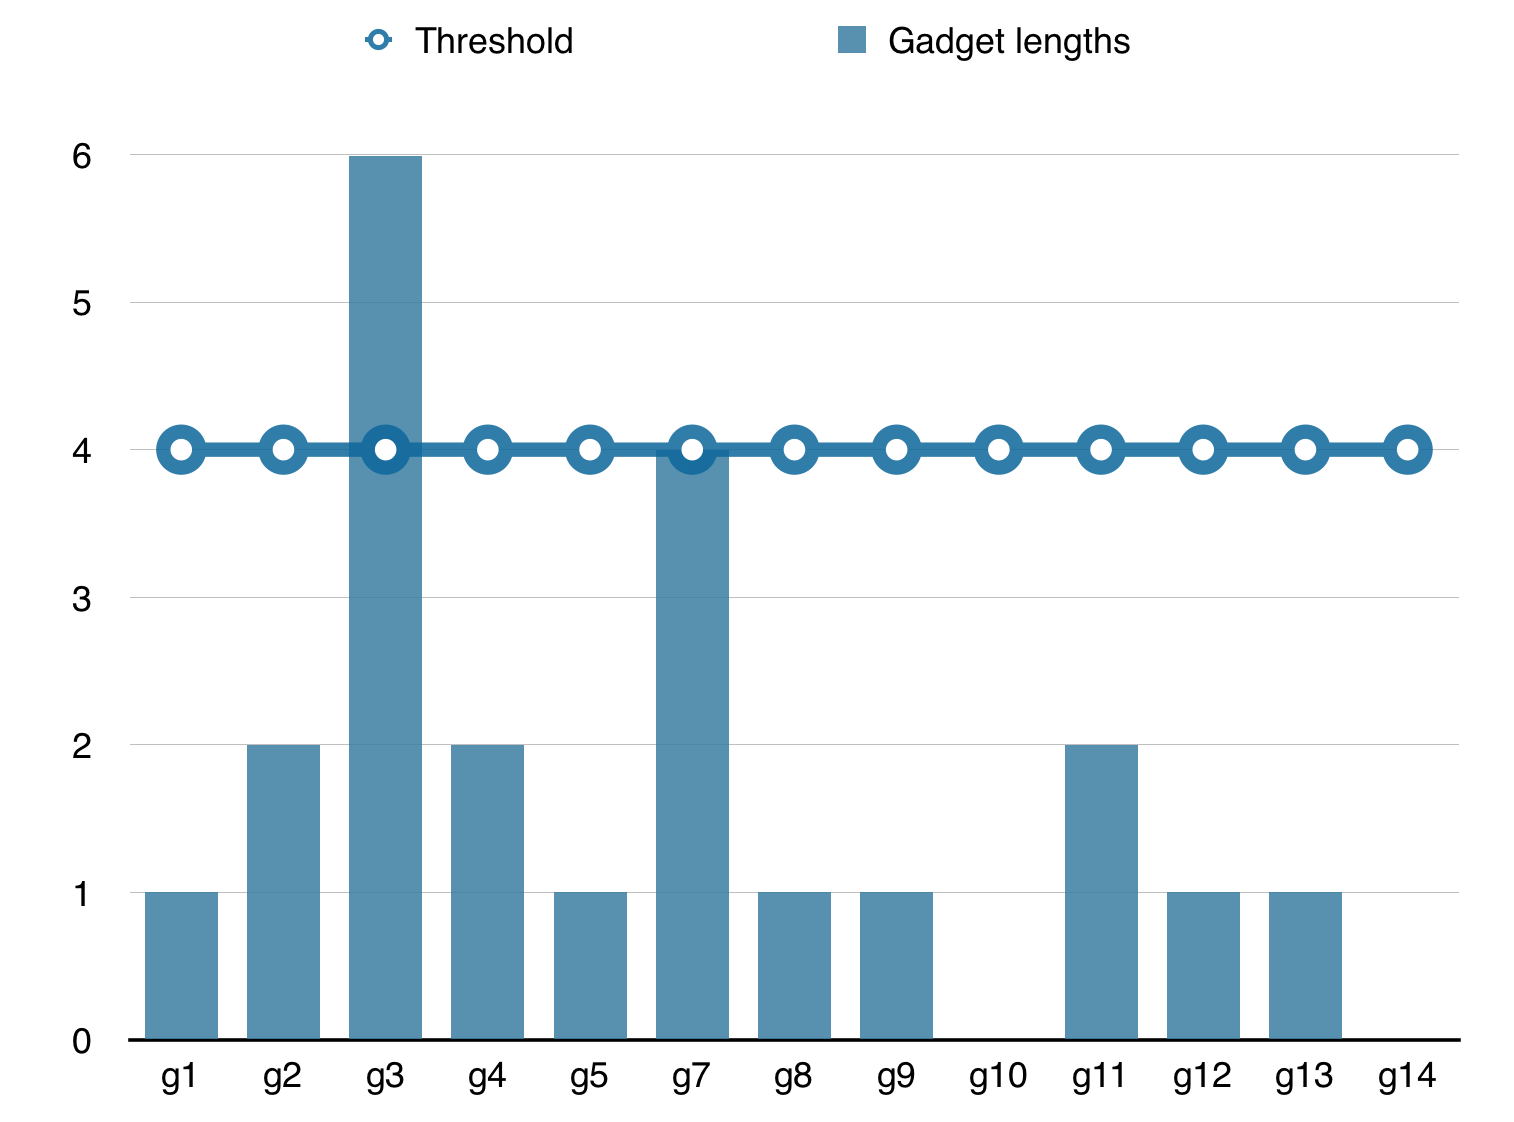
\includegraphics[width=1\textwidth]{params}
\caption{Ret-to-libc: stack configuration right before the call to libc function}
\label{fig:largenenough}
\end{figure}

\chapter{Evaluation}

\section{Testing environment}
To evaluate our work we run the tool on multiple real world applications. In some of them we only wanted to make sure that the tool doesn’t stop the regular flow of execution detecting false positives. Our tool is not OS specific, however we chose to target Windows vulnerable applications for the tests, since there is a wider range of recorded exploits to reproduce. In particular we selected exploits working on a Windows 7 (build 7601) environment. The reason of the choice is twofold: first Windows XP is not longer supported by Microsoft, and does not receive protection updates any more, second the default DEP policies on Windows 7 are the same in higher versions. Of course since the exploits rely on the presence and semantics of particular system APIs, the attacks could not work on these higher versions.

\section{What we learned from tests}

The version 1.0 of the tool was tested on every day use applications to check that no false positives are detected. These applications include Adobe Acrobat Reader, Internet Explorer 8, the Microsoft Office Suite 2016 (Word, Excel, PowerPoint, Access, Outlook, Publisher). The first problems occurred with the Google Chrome and Mozilla Firefox browsers. In particular analysing the traces of disassembled executions some really peculiar code behaviours came up. These traces were generated by another Pin tool that employed the INS\_Disassemble() and other facilities from the Pin framework. The false positives that version 1.0 found were of this form in Firefox:
\begingroup
    \fontsize{8pt}{9pt}\selectfont
\begin{verbatim}

0x56500d10 C:\cygwin\home\Mozilla Firefox\xul.dll:.text+0x6b50			mov ecx, dword ptr [esp+0x5c]
0x56500d14 C:\cygwin\home\Mozilla Firefox\xul.dll:.text+0x6b54         jmp 0x565008b0
0x569c1010 C:\cygwin\home\Mozilla Firefox\xul.dll:.text+0x2310         mov eax, 0x104
0x569c1015 C:\cygwin\home\Mozilla Firefox\xul.dll:.text+0x2315         ret 
0x569d4200 C:\cygwin\home\Mozilla Firefox\xul.dll:.text+0x15500        mov eax, 0x7e
0x569d4205 C:\cygwin\home\Mozilla Firefox\xul.dll:.text+0x15505        ret 
0x569d4200 C:\cygwin\home\Mozilla Firefox\xul.dll:.text+0x15500        mov eax, 0x7e
0x569d4205 C:\cygwin\home\Mozilla Firefox\xul.dll:.text+0x15505        ret 
0x569d5470 C:\cygwin\home\Mozilla Firefox\xul.dll:.text+0x16770        mov eax, 0x11c
0x569d5475 C:\cygwin\home\Mozilla Firefox\xul.dll:.text+0x16775        ret 
0x569d30e0 C:\cygwin\home\Mozilla Firefox\xul.dll:.text+0x143e0        mov eax, 0x112
0x569d30e5 C:\cygwin\home\Mozilla Firefox\xul.dll:.text+0x143e5        ret 
0x569d2ce0 C:\cygwin\home\Mozilla Firefox\xul.dll:.text+0x13fe0        mov eax, 0x3
0x569d2ce5 C:\cygwin\home\Mozilla Firefox\xul.dll:.text+0x13fe5        ret 
0x569d5490 C:\cygwin\home\Mozilla Firefox\xul.dll:.text+0x16790        mov eax, 0x73
0x569d5495 C:\cygwin\home\Mozilla Firefox\xul.dll:.text+0x16795        ret 
0x569d3170 C:\cygwin\home\Mozilla Firefox\xul.dll:.text+0x14470        mov eax, 0xf3
0x569d3175 C:\cygwin\home\Mozilla Firefox\xul.dll:.text+0x14475        ret 
0x569d5470 C:\cygwin\home\Mozilla Firefox\xul.dll:.text+0x16770        mov eax, 0x11c
0x569d5475 C:\cygwin\home\Mozilla Firefox\xul.dll:.text+0x16775        ret 
0x569d30b0 C:\cygwin\home\Mozilla Firefox\xul.dll:.text+0x143b0        mov eax, 0xf7
0x569d30b5 C:\cygwin\home\Mozilla Firefox\xul.dll:.text+0x143b5        ret 
0x569d4200 C:\cygwin\home\Mozilla Firefox\xul.dll:.text+0x15500        mov eax, 0x7e
0x569d4205 C:\cygwin\home\Mozilla Firefox\xul.dll:.text+0x15505        ret 
0x56887ef8 C:\cygwin\home\Mozilla Firefox\xul.dll:.text+0x1eeb8        cmp esi, dword ptr [eax]
0x56887efa C:\cygwin\home\Mozilla Firefox\xul.dll:.text+0x1eeba        jz 0x56887f07
0x56887efc C:\cygwin\home\Mozilla Firefox\xul.dll:.text+0x1eebc        xor eax, eax
0x56887efe C:\cygwin\home\Mozilla Firefox\xul.dll:.text+0x1eebe        pop edi
0x56887eff C:\cygwin\home\Mozilla Firefox\xul.dll:.text+0x1eebf        pop esi
0x56887f00 C:\cygwin\home\Mozilla Firefox\xul.dll:.text+0x1eec0        pop ebx
0x56887f01 C:\cygwin\home\Mozilla Firefox\xul.dll:.text+0x1eec1        mov esp, ebp
0x56887f03 C:\cygwin\home\Mozilla Firefox\xul.dll:.text+0x1eec3        pop ebp
0x56887f04 C:\cygwin\home\Mozilla Firefox\xul.dll:.text+0x1eec4        ret 0x8
0x564ff640 C:\cygwin\home\Mozilla Firefox\xul.dll:.text+0x5480         mov eax, 0x175
0x564ff645 C:\cygwin\home\Mozilla Firefox\xul.dll:.text+0x5485         ret 

\end{verbatim}
\endgroup
And similarly in Chrome:

\begingroup
    \fontsize{8pt}{9pt}\selectfont
\begin{verbatim}

0x62ab4775 C:\...\Chrome\Application\60.0.3112.113\chrome.dll:.text+0x0eb5        call 0x623a1cdc
0x62ab513c C:\...\Chrome\Application\60.0.3112.113\chrome.dll:.text+0x187c        mov eax, 0x6336ffa0
0x62ab5141 C:\...\Chrome\Application\60.0.3112.113\chrome.dll:.text+0x1881        ret 
0x62ab5142 C:\...\Chrome\Application\60.0.3112.113\chrome.dll:.text+0x1882        mov eax, 0x63370124
0x62ab5147 C:\...\Chrome\Application\60.0.3112.113\chrome.dll:.text+0x1887        ret 
0x62ab5148 C:\...\Chrome\Application\60.0.3112.113\chrome.dll:.text+0x1888        mov eax, 0x6336ff60
0x62ab514d C:\...\Chrome\Application\60.0.3112.113\chrome.dll:.text+0x188d        ret 
0x62ab514e C:\...\Chrome\Application\60.0.3112.113\chrome.dll:.text+0x188e        mov eax, 0x6336fe5c
0x62ab5153 C:\...\Chrome\Application\60.0.3112.113\chrome.dll:.text+0x1893        ret 
0x62ab5154 C:\...\Chrome\Application\60.0.3112.113\chrome.dll:.text+0x1894        mov eax, 0x6336ffb0
0x62ab5159 C:\...\Chrome\Application\60.0.3112.113\chrome.dll:.text+0x1899        ret 
0x62ab515a C:\...\Chrome\Application\60.0.3112.113\chrome.dll:.text+0x189a        mov eax, 0x6337020c
0x62ab515f C:\...\Chrome\Application\60.0.3112.113\chrome.dll:.text+0x189f        ret 
0x62ab5160 C:\...\Chrome\Application\60.0.3112.113\chrome.dll:.text+0x18a0        mov eax, 0x63370074
0x62ab5165 C:\...\Chrome\Application\60.0.3112.113\chrome.dll:.text+0x18a5        ret 
0x62ab5166 C:\...\Chrome\Application\60.0.3112.113\chrome.dll:.text+0x18a6        mov eax, 0x6336fe34
0x62ab516b C:\...\Chrome\Application\60.0.3112.113\chrome.dll:.text+0x18ab        ret 
0x62ab516c C:\...\Chrome\Application\60.0.3112.113\chrome.dll:.text+0x18ac        mov eax, 0x6336ff28
0x62ab5171 C:\...\Chrome\Application\60.0.3112.113\chrome.dll:.text+0x18b1        ret 
0x62ab5172 C:\...\Chrome\Application\60.0.3112.113\chrome.dll:.text+0x18b2        mov eax, 0x63370218
0x62ab5177 C:\...\Chrome\Application\60.0.3112.113\chrome.dll:.text+0x18b7        ret 
0x62ab5178 C:\...\Chrome\Application\60.0.3112.113\chrome.dll:.text+0x18b8        mov eax, 0x6336fe88
0x62ab517d C:\...\Chrome\Application\60.0.3112.113\chrome.dll:.text+0x18bd        ret 
0x62ab517e C:\...\Chrome\Application\60.0.3112.113\chrome.dll:.text+0x18be        mov eax, 0x6336fdd8
0x62ab5183 C:\...\Chrome\Application\60.0.3112.113\chrome.dll:.text+0x18c3        ret 
0x62ab5184 C:\...\Chrome\Application\60.0.3112.113\chrome.dll:.text+0x18c4        mov eax, 0x633700c0
0x62ab5189 C:\...\Chrome\Application\60.0.3112.113\chrome.dll:.text+0x18c9        ret 
0x62ab518a C:\...\Chrome\Application\60.0.3112.113\chrome.dll:.text+0x18ca        mov eax, 0x6336ffe8
0x62ab518f C:\...\Chrome\Application\60.0.3112.113\chrome.dll:.text+0x18cf        ret 
0x62ab5190 C:\...\Chrome\Application\60.0.3112.113\chrome.dll:.text+0x18d0        mov eax, 0x6336fe94
0x62ab5195 C:\...\Chrome\Application\60.0.3112.113\chrome.dll:.text+0x18d5        ret 
0x62ab5196 C:\...\Chrome\Application\60.0.3112.113\chrome.dll:.text+0x18d6        mov eax, 0x633701d0
0x62ab519b C:\...\Chrome\Application\60.0.3112.113\chrome.dll:.text+0x18db        ret 
0x62ab519c C:\...\Chrome\Application\60.0.3112.113\chrome.dll:.text+0x18dc        mov eax, 0x6336ff3c
0x62ab51a1 C:\...\Chrome\Application\60.0.3112.113\chrome.dll:.text+0x18e1        ret 

\end{verbatim}
\endgroup

This kind of problem was solved by carefully choosing a threshold in the distance between the addresses of the ret instructions, in fact you can see that in these traces the most significant digits are the same among the consecutive rets that are very close to each other.
Another important part of the evaluation was testing the detection on real world exploits based on ROP. To accomplish this we used two vulnerable applications available in the exploit-db.com database:
\begin{itemize}
\item
https://www.exploit-db.com/exploits/20116/ RM-MP3 Converter 3.1.2.1. In this case another lighter and more efficient version of attack was used rather than the one in the database.
\item
https://www.exploit-db.com/exploits/13763/ Audio-Converter 8.1, even in this case we used another attack taken from: http://tekwizz123.blogspot.it/2014/02\\ /bypassing-aslr-and-dep-on-windows-7.html
\end{itemize}
Both the exploits try to create the right stack configuration and to craft the right arguments in order to do a successful call to VirtualAlloc. After that, the code tries to launch a shellcode given in the input payload. 
In RM-MP3 converter the output of the tool is the following. We can notice that the structure of the attack is forecast earlier than the moment where the process is terminated (notice that the numbers of the list are sliding from right to left in the various detections and that the percentage of short intervals increases), but the tool waits and verifies that this can’t be regular code checking the distances in terms of addresses of the various suspected gadgets.

\begin{verbatim}

short intervals: 78.5714%
super short intervals: 57.1429%
10 10 0 1 1 2 1 1 1 1 5 2 1 2


short intervals: 85.7143%
super short intervals: 64.2857%
10 0 1 1 2 1 1 1 1 5 2 1 2 0


short intervals: 92.8571%
super short intervals: 71.4286%
0 1 1 2 1 1 1 1 5 2 1 2 0 1


short intervals: 92.8571%
super short intervals: 64.2857%
1 1 2 1 1 1 1 5 2 1 2 0 1 2


short intervals: 92.8571%
super short intervals: 57.1429%
1 2 1 1 1 1 5 2 1 2 0 1 2 2


short intervals: 92.8571%
super short intervals: 57.1429%
2 1 1 1 1 5 2 1 2 0 1 2 2 1

===========================================
!!! Too short intervals !!!
short intervals: 92.8571%
super short intervals: 64.2857%
1 1 1 1 5 2 1 2 0 1 2 2 1 1
===========================================
*******************************************************
!!! Too far instructions !!!
large distances: 50%
*******************************************************
ROP DETECTED!
Terminating Program...

\end{verbatim}



In the Audio-Converter application instead the output of the tool is the following. As you can see the attack is very condensed in a short sequence of gadgets, but compared to the RM-MP3 exploit, here the gadgets are more scattered, in fact the percentage of rets that are at a distance greater than the threshold is 100\%.

\begin{verbatim}

=======================================================
This application is analysed by RopDetect
=======================================================
!!! Too short intervals !!!
short intervals: 78.5714%
super short intervals: 78.5714%
1 1 1 1 1 1 1 1 1 1 0 190 290 45
=======================================================
*******************************************************
!!! Too far instructions !!!
large distances: 100%
*******************************************************
ROP DETECTED!
Exiting Program...

\end{verbatim}

We will not discuss the details of the code used to generate the exploiting input nor we will review the fundamentals of shellcode writing since it is beyond the scope of this work. However if you are a curious reader, in the GitHub repository (https://github.com/spallas/ropbuster) in the directory test/ you can find an abundantly commented code used to generate the malformed inputs that cause the buffer overflows and that carry out the ROP attack, together with the vulnerable executables of the two applications.


\chapter{Conclusions and Related work}

\section{Possible future improvements}

The current version of the tool is actually rather simple. It’s composed of some heuristics that try to catch the underlying characteristics of ROP code, avoiding as much as possible to incur in false positives. The tool can be improved making the detection logic more sophisticated, and more aware about the semantics of the execution under analysis. For example in the false positives given in paragraph [Evaluation] you can notice that the code that can be confused with ROP by the tool, is actually doing the same operation multiple times with different data, without a real articulated computation underneath, so we could check that the code under test is actually doing something interesting and potentially harmful. At the same time as other works pointed out, almost all the real world ROP attacks use this technique to disable DEP/WxorX, in order to execute shellcode, so a more efficient check could be accomplished through API hooking. This technique consists in adding some code to be executed every time a system call is invoked so that you can add additional security checks before running dangerous functions, like in our case VirtualAlloc() or VirtualProtect(). However, even if really practical, this idea doesn’t acknowledge the real essence of ROP attacks that can be completely independent in theory from the DEP protections and configurations.


One of the greatest limits of our work is performance. A program running with the Pin framework instructions instrumentation is much slower than in normal conditions. In fact since every single instruction is analysed by the callback routines, for example to check if the instruction is a ret or not, the weight of the execution on the processor and memory is multiplied by a k factor. However since the algorithms are not too complicated some hardware solutions can be devised. For example, like other defences do, we could employ the LBR (Last Branch Record) register, but we would be exposed to the same problems other researcher met, included LBR flush gadget sequences and problems with multicore and multithreaded applications.

\backmatter
% bibliography
%\cleardoublepage
%\phantomsection
%\bibliographystyle{sapthesis} % BibTeX style
%\bibliography{bibliography} % BibTeX database without .bib extension

\end{document}
